\documentclass[journal, a4paper]{IEEEtran}
% \documentclass[12pt, a4paper, oneside]{ctexart}

% some very useful LaTeX packages include:

\usepackage{ctex}
\usepackage{graphicx}
\usepackage{animate}
\usepackage{subfigure}
\usepackage{url}
\usepackage{amssymb}
\usepackage{amsmath}
\usepackage{cite}
\usepackage{multirow}
\usepackage{listings}
\usepackage{booktabs}
\usepackage[colorlinks,linkcolor=blue]{hyperref}
\usepackage{listings}
% \usepackage{xcolor}
\usepackage{float}
\usepackage{hyperref}
\usepackage{caption}
\usepackage{algorithm}
\usepackage{algpseudocode}
\usepackage[table,xcdraw]{xcolor}

\lstset{
    columns=fixed,
    frame=none,
    keywordstyle=\color[RGB]{40,40,255},
    numberstyle=\footnotesize\color{darkgray},
    commentstyle=\it\color[RGB]{0,96,96},
    stringstyle=\rmfamily\slshape\color[RGB]{128,0,0},
    showstringspaces=false,
    tabsize=4
}

% Your document starts here!
\begin{document}

\newcommand{\figref}[1]{图\ref{#1}}
\newcommand{\tabref}[1]{表\ref{#1}}
\newcommand{\equref}[1]{式\ref{#1}}
\newcommand{\secref}[1]{第\ref{#1}节}

% Define document title and author
\title{\textbf{Group LASSO Problem 编程作业报告}}
\author{李锦韬$^*$ 2201213292
\thanks{$*$ e-mail: lijintao@stu.pku.edu.cn \\ \url{https://github.com/AkexStar/Algorithms-group-LASSO-problem}}}
\markboth{最优化方法 2023 秋季学期 }{}
\maketitle
% \begin{abstract}
%     摘要测试
% \end{abstract}

% \begin{keywords}
% 	Authors shall provide a maximum of six keywords (in alphabetical order, capitalized, separated by commas) to help identify the major topics of the paper.
% \end{keywords}

% Main Part

\begin{table*}[h!]
\caption{所有算法的求解结果对比}
\centering
\begin{tabular}{lcccccccc}
\hline
\textbf{Solver} & \textbf{Obj} & \textbf{Obj\_ABS\_Error} & \textbf{x\_u\_Err} & \textbf{x\_mosek\_Err} & \textbf{x\_gurobi\_Err} & \textbf{Time(s)} & \textbf{Iter} & \textbf{Sparsity} \\ \hline
cvx\_mosek      & 0.652291     & 1.3621E-05               & 3.9124E-05         & 0                      & 2.0631E-06              & 0.468511         & 13            & 0.102539          \\
cvx\_gurobi     & 0.652291     & 1.3355E-05               & 3.7553E-05         & 2.0631E-06             & 0                       & 0.828498         & 12            & 0.102539          \\
mosek           & 0.652301     & 3.3387E-06               & 9.8422E-06         & 2.9283E-05             & 2.7719E-05              & 0.362566         & 11            & 0.099609          \\
gurobi          & 0.652291     & 1.3373E-05               & 3.9706E-05         & 8.2778E-07             & 2.5405E-06              & 0.591821         & 13            & 0.103516          \\
SGD\_primal     & 0.652294     & 1.0286E-05               & 5.5248E-05         & 1.8991E-05             & 2.0386E-05              & 0.724858         & 1473          & 0.121094          \\
ProxGD\_primal  & 0.652291     & 1.3642E-05               & 3.8956E-05         & 3.1614E-07             & 1.9959E-06              & 0.179088         & 190           & 0.102539          \\
FProxGD\_primal & 0.652291     & 1.3642E-05               & 3.8964E-05         & 3.1193E-07             & 2.0041E-06              & 0.250055         & 486           & 0.102539          \\
ALM\_dual       & 0.652308     & 3.9728E-06               & 6.8346E-05         & 3.6216E-05             & 3.7335E-05              & 0.228689         & 70            & 0.099609          \\
ADMM\_dual      & 0.652309     & 4.8089E-06               & 6.8479E-05         & 3.6551E-05             & 3.7576E-05              & 0.071023         & 86            & 0.099609          \\
ADMM\_primal    & 0.652291     & 1.3476E-05               & 3.8987E-05         & 3.0987E-07             & 2.0185E-06              & 0.616442         & 2694          & 0.102539          \\ \hline
\end{tabular}
\label{tab:all}
\newline \\
% {'seed': 97108120, 'mu': 0.01, 'n': 512, 'm': 256, 'l': 2, 'r': 0.1}
\raggedright
\footnotesize 
注1:精确解的目标函数值为 $0.6523043$,稀疏度为 $0.09960937$。
\newline
注2:数据生成时,随机数种子为 $97108120$,正则化参数 $\mu = 0.01$,矩阵 $A$ 的维度为 $256 \times 512$,矩阵 $b$ 的维度为 $256 \times 2$,矩阵 $x$ 的维度为 $512 \times 2$,矩阵 $x$ 的稀疏度为 $0.1$。
\newline
注3:求解器 \texttt{cvx\_mosek} 和 \texttt{cvx\_gurobi} 为 CVX 直接调用 Mosek 和 Gurobi 求解器求解得到的结果,求解器 \texttt{mosek} 和 \texttt{gurobi} 为直接调用 Mosek 和 Gurobi 求解器求解得到的结果。
\end{table*}

\section{\textbf{问题描述}}
算法需要求解的Group LASSO问题为:
\begin{equation}\label{eq:prob}
    \min _{x \in \mathbb{R}^{n \times l}} \frac{1}{2}\|A x-b\|_F^2+\mu\|x\|_{1,2}
\end{equation}
其中 $A \in \mathbb{R}^{m \times n}$, $b \in \mathbb{R}^{m \times l}$, $\mu>0$ 并且
$$
\|x\|_{1,2}=\sum_{i=1}^n\|x_{(i, 1: l)}\|_2
$$
其中 $x_{(i, 1: l)}$ 是矩阵 $x$ 的第 $i$ 行。

\section{\textbf{评价指标}}

项目完成了多个算法的实现,为了实现不同结果效率之间的对比,本项目将使用以下指标\cite{wzwProblem}来评价各个算法的性能。

\begin{itemize}
    \item \texttt{Obj\_ABS\_Err}:算法得到的最终目标函数值 和 最优解对应的目标函数 之间的绝对值差:
    $$
    Error(f_{x}, f_{u}) = |f_{x} - f_{u}|
    $$
    其中 $f_{x}$ 为算法得到的最终目标函数值,$f_{u}$ 为最优解 $u$ 对应的目标函数值。

    \item \texttt{x\_u\_Err}:算法得到的最终解 和 最优解 之间的 归一化范数差:
    $$
    Error(x, u) = \frac{\|x - u\|_F}{1 + \|u\|_F}
    $$
    其中 $x$ 为算法得到的最终解,$u$ 为最优解。

    \item \texttt{x\_mosek\_Err}:算法得到的最终解与 CVX-mosek 所得解之间的归一化范数差:
    $$
    Error(x, x_{cvx}) = \frac{\|x - x_{cvx}\|_F}{1 + \|x_{cvx}\|_F}
    $$

    其中 $x$ 为算法得到的最终解,$x_{cvx}$ 为使用 CVXPY 调用 Mosek 或 Gurobi 求解得到的最优解。
    \item \texttt{x\_gurobi\_Err}:算法得到的最终解与 CVX-Gurobi 所得解之间的归一化范数差:
    $$
    Sparsity = \frac{\|x\|_0}{n \times l}
    $$

    其中 $x$ 为算法得到的最终解,$\|x\|_0$ 表示 $x$ 中非零元素的个数,在本项目中认为绝对值小于 $10^{-5}$ 的元素为零。

    \item \texttt{Obj}:算法得到的最终目标函数值。
    \item \texttt{Time(s)}:算法求解的运行时间。
    \item \texttt{Iter}:算法求解的迭代次数。
    \item \texttt{Sparsity}:算法得到的最终解的稀疏度。
\end{itemize}

\section{\textbf{CVX直接求解}}
使用 CVX 软件包可以直接求解\ref{eq:prob}所描述的问题,无需变换形式。项目使用 CVX 的 python 版本,即 CVXPY,其版本信息已在README中说明。
CVX 记录的迭代信息是通过 \texttt{verbose=True} 来实现的,由于其无法直接被读取和存储,本项目使用重定向 \texttt{stdout} 的技巧\cite{stackoverflow},使其将输出信息记录在文本文件,再采用正则表达式匹配的方式从中提取每一次迭代的数据。

由\tabref{tab:all}和\figref{fig:CVX1}可知:
\begin{itemize}
    \item CVX 调用 Mosek 和 Gurobi 求解器的效率相当,但 Mosek 用时更少,只有 Gurobi 用时的一半,而Gurobi从初值收敛更快。
    \item Mosek 和 Gurobi 得到的解非常相似,数值上几乎相同,稀疏度也基本一致。
    \item Gurobi 在第一次迭代中出现负目标函数值,这可能是由于求解器的初始求解策略所致。
\end{itemize}

\begin{figure}[H]
    \centering
    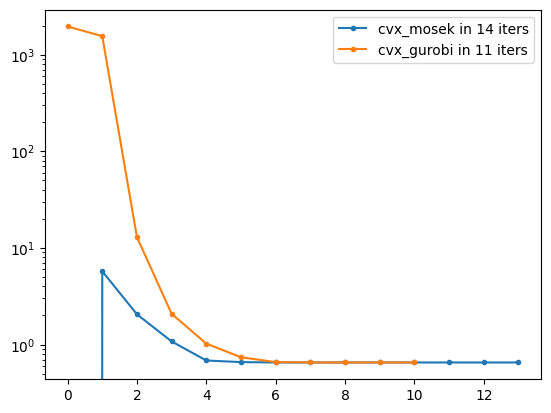
\includegraphics[width=0.8\columnwidth]{img/cvx-mosek-gurobi.png}
    {\centering \small \caption{CVX 直接调用求解结果\label{fig:CVX1}}}
\end{figure}

\begin{figure*}[htbp]
    \centering
    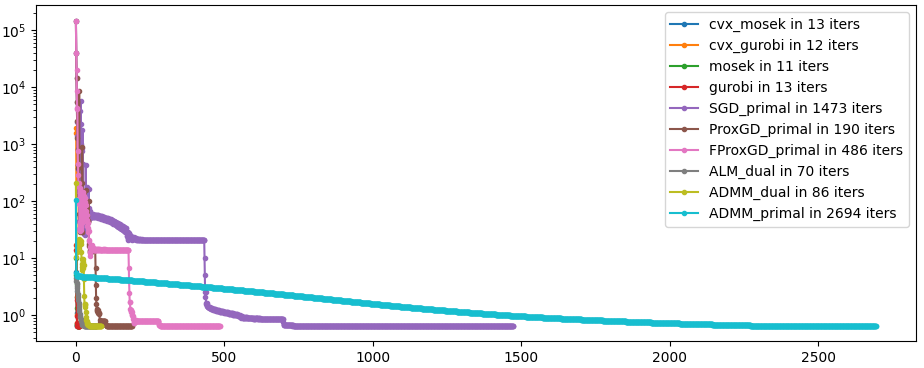
\includegraphics[width=1.7\columnwidth]{img/test-all.png    }
    {\centering \small \caption{所有算法的目标函数下降迭代图\label{fig:all}}}
\end{figure*}

\section{\textbf{直接调用Mosek和Gurobi求解}}
Mosek 和 gurobi 同样拥具备对应的 python 软件包,可以直接调用。但是由于其要求问题形式必须为所谓标准形式,因此需要对原问题进行变换。

\subsection{\textbf{Mosek}}

对于 Mosek,原问题转换为如下形式:
\begin{align*}
    & \underset{t, z}{\min} & & \frac{1}{2} t + \mu \sum_{i=1}^{n} z_i \\
    & \text{s.t.} & & Ax - b = y \\
    & & & \begin{bmatrix}
        1 + t \\
        2 \times \text{vec}(y) \\
        1 - t
    \end{bmatrix} \in \mathcal{Q} \\
    & & & \begin{bmatrix}
        z_i \\
        (x_{(i,:)})^T
    \end{bmatrix} \in \mathcal{Q}, \quad \forall i = 1, \ldots, n
\end{align*}
其中 $\mathcal{Q}$ 表示二次锥(Second-Order Cone,SOC),写作$\mathcal{Q}_{\text{SOC}} = \{(t, x) \mid \lVert x \rVert_2 \leq t, \; t \geq 0\}$,$\text{vec}(y)$ 表示矩阵 $y$ 的向量化,$x_{(i,:)}$ 表示矩阵 $x$ 的第 $i$ 行。

代码实现在 \texttt{gl\_mosek.py} 中给出,其主要思路为:
\begin{itemize}
    \item 使用 \texttt{Model} 类创建模型。
    \item 使用 \texttt{Variable} 方法添加变量。
    \item 使用 \texttt{Constraint} 方法添加约束。
    \item 使用 \texttt{Objective} 方法设置目标函数。
    \item 使用 \texttt{solve} 方法求解。
\end{itemize}

\subsection{\textbf{Gurobi}}
Gurobi 同理,但不用写成二次锥约束的形式,第一项范数中的部分可以整个做变量替换,而第二项需要把范数替换成新的变量,原问题转换为如下形式:
\begin{align*}
    & \underset{y, z}{\min} & & \frac{1}{2} \|y\|_F^2 + \mu \sum_{i=1}^{n} z_i \\
    & \text{s.t.} & & Ax - b = y \\
    & & & \|x_{(i, : )}\|_2 \leq z_i, \quad \forall i = 1, \ldots, n
\end{align*}
其中 $x_{(i,:)}$ 表示矩阵 $x$ 的第 $i$ 行。

代码实现在 \texttt{gl\_gurobi.py} 中给出,其主要思路为:
\begin{itemize}
    \item 使用 \texttt{Model} 类创建模型。
    \item 使用 \texttt{addVars} 方法添加变量。
    \item 使用 \texttt{addConstrs} 方法添加约束。
    \item 使用 \texttt{setObjective} 方法设置目标函数。
    \item 使用 \texttt{optimize} 方法求解。
\end{itemize}

\subsection{\textbf{Mosek和Gurobi求解结果}}

由\tabref{tab:all}和\figref{fig:MosekGurobi}可知:

\begin{itemize}
    \item Mosek 和 Gurobi 求解器的效率相当,迭代次数甚至相同。
    \item Gurobi 在第一次迭代中出现负目标函数值,这可能是由于求解器的初始求解策略所致。
    \item Mosek 和 Gurobi 得到的解与 CVX 得到的解非常相似,数值上几乎相同。
\end{itemize}

\begin{figure}[H]
    \centering
    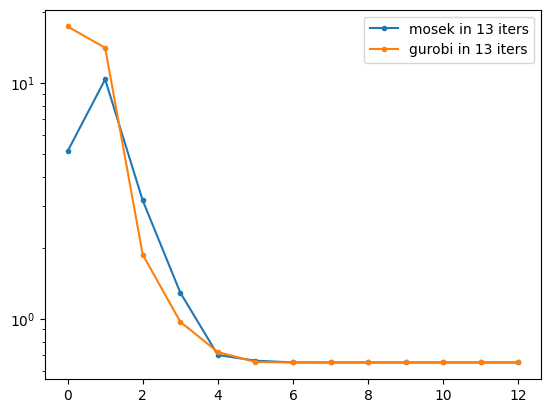
\includegraphics[width=0.8\columnwidth]{img/mosek-gurobi.png}
    {\centering \small \caption{Mosek 和 Gurobi 求解结果}\label{fig:MosekGurobi}}
    
\end{figure}

\section{\textbf{连续化策略}}

对于本项目 LASSO 问题,即\ref{eq:prob},连续化策略从较大的正则化参数 $\mu_t$ 逐渐减小到 $\mu_0$(即 $\mu_1 \geq \ldots \geq \mu_{t-1} \geq \mu_t \geq \ldots \geq \mu_0$),并求解相应的新的 LASSO 问题:
\begin{equation}\label{eq:prob-mut}
    \min _{x \in \mathbb{R}^{n \times l}} \frac{1}{2}\|A x-b\|_F^2+\mu_{t}\|x\|_{1,2}
\end{equation}

这样做的好处是:在求解 $\mu_t$ 对应的优化问题时,可以利用 $\mu_{t-1}$ 对应优化问题的解($\mu_1$ 子问题使用随机初始点)作为一个很好的逼近解以在较短的时间内完成求解过程;分析可知 $\mu_t$ 越大,相应的 LASSO 问题越好解\cite{LASSO_con}。因此,连续化策略相当于是通过快速求解一系列简单问题(复杂问题有了好的初始解也就变简单了)来加速求解原始问题。

在调用迭代算法求解 $\mu_t$ 对应的 LASSO 问题后,正则化参数 $\mu_{t+1}$ 的更新公式取为:
$$
\mu_{t+1} = \max\{\mu_0, \mu_t \eta\}
$$
其中 $\eta \in (0,1)$ 为一个缩小因子。

在本项目中,SGD算法、ProxGD算法、FProxGD算法均可使用连续化策略进行加速,相当于在每个求解器外部再套一层循环,每次循环中调用求解器求解一个新的 LASSO 问题。

具体而言,本项目原问题中$\mu_0$ 为 $0.01$,本项目选取$\mu_1$ 为 $100$,$\eta$ 取为 $0.1$。

\section{\textbf{SGD次梯度算法}}

\subsection{\textbf{算法描述}}
次梯度算法是梯度法的一种泛化形式,通过使用次梯度来代替梯度,从而允许处理本问题目标函数中第二个非光滑项。其算法描述的伪代码如算法\ref{alg:SGD}所示。

\begin{algorithm}
    \caption{SGD Solver}
    \label{alg:SGD}
    \begin{algorithmic}[1]
    \State \textbf{Input:} $A \in \mathbb{R}^{m \times n}$, $b \in \mathbb{R}^{m \times l}$, $\mu > 0$, maximum iterations \texttt{max\_iter}, tolerance \texttt{tol}
    \State Initialize $x^{(0)}$ (random initialization)
    \State Set Lipschitz constant $L$ (e.g., $L = \lVert A^TA \rVert_2$)
    \For{$k = 0, 1, 2, \ldots, \texttt{max\_iter}$}
        \State Compute subgradient $g^{(k)}$:
        \[
        g^{(k)} = A^T(Ax^{(k)} - b) + \mu \cdot \partial_{\ell_{1,2}}(x^{(k)})
        \]
        \State Update $x^{(k+1)}$ using proximal operator:
        \[
        x^{(k+1)} = \text{prox}_{\frac{1}{L}\mu\lVert \cdot \rVert_{1,2}}\left(x^{(k)} - \frac{1}{L} g^{(k)}\right)
        \]
        \State Check convergence: if $\lVert x^{(k+1)} - x^{(k)} \rVert_F < \texttt{tol}$, break
    \EndFor
    \State \textbf{Output:} $x^{(k+1)}$
    \end{algorithmic}
\end{algorithm}

\subsection{\textbf{算法实现}}

针对本项目中的问题,次梯度算法的实现关键在于如何计算 $\partial_{\ell_{1,2}}(x^{(k)})$。由于 $\ell_{1,2}$ 范数的定义为:
\begin{equation*}\label{eq:l12}
    \lVert x \rVert_{1,2} = \sum_{i=1}^{n} \lVert x_{(i, :)} \rVert_2
\end{equation*}
其中 $x_{(i, :)}$ 表示矩阵 $x$ 的第 $i$ 行。因此,可以将 $\partial_{\ell_{1,2}}(x^{(k)})$ 分解为:
\begin{equation*}\label{eq:subgrad}
    \partial_{\ell_{1,2}}(x^{(k)}) = \sum_{i=1}^{n} \partial_{\ell_2}(x_{(i, :)}^{(k)})
\end{equation*}
其中 $\partial_{\ell_2}(x_{(i, :)}^{(k)})$ 表示 $\ell_2$ 范数的次梯度,其定义为:
\begin{equation*}\label{eq:l2subgrad}
    \partial_{\ell_2}(x_{(i, :)}^{(k)}) = \begin{cases}
        \frac{x_{(i, :)}^{(k)}}{\lVert x_{(i, :)}^{(k)} \rVert_2} & \text{if } x_{(i, :)}^{(k)} \neq 0 \\
        \text{any } v \in \mathbb{R}^l \text{ with } \lVert v \rVert_2 \leq 1 & \text{if } x_{(i, :)}^{(k)} = 0
    \end{cases}
\end{equation*}


\subsection{\textbf{算法结果}}

\section{\textbf{ProxGD次梯度算法}}

对于上述目标函数,近似点梯度法考虑令 $\phi(x)=\frac{1}{2}\|Ax-b\|_2^2$,$h(x)=\mu\|x\|_1$,对光滑部分做梯度下降,并对非光滑部分使用近似点算子,得到迭代格式 $x_{k+1}=\text{prox}_{tkh(\cdot)}(x_k-t_k\nabla\phi(x_k))$。

在此问题中,近似点算子可以解析地写出:

\subsection{\textbf{算法描述}}

\subsection{\textbf{算法实现}}

\subsection{\textbf{算法结果}}

\section{\textbf{FProxGD次梯度算法}}




\bibliographystyle{IEEEtran}
\bibliography{main}


% Your document ends here!
\end{document}